\newcommand\user[2]{
	\begin{scope}[xshift=#1cm, yshift=#2cm]
		\clip (0, 0) circle (0.5);
		\fill[black] (0, 0) circle (0.5);
		\fill[white] (0, 0) circle (0.48);
		\fill[black] (0, -0.675) circle (0.4);
		\fill[black] (0, 0.075) circle (0.24);
	\end{scope}
}

\newcommand\ip[2]{
	\begin{scope}[xshift=#1cm, yshift=#2cm]
		%\rectangle[fill=black, rounded corners=0.2cm] (-0.5, -0.7) -- (0.5, 0.7);
		\draw[fill=black, thick, rounded corners=0.15cm] (-0.3, -0.5) rectangle (0.3, 0.5);
		\draw[fill=white] (0, -0.3) circle (0.1);
		\draw[fill=white, rounded corners=0.07cm] (-0.2, -0.1) rectangle (0.2, 0.0);
		\draw[fill=white, rounded corners=0.07cm] (-0.2, 0.1) rectangle (0.2, 0.2);
		\draw[fill=white, rounded corners=0.07cm] (-0.2, 0.3) rectangle (0.2, 0.4);
	\end{scope}
}

\newcommand\www[2]{
	\begin{scope}[xshift=#1cm, yshift=#2cm]
		\clip (0, 0) circle (0.5);
		\fill[yellow!65!black] (0, 0) circle (0.5);
		\fill[white] (-0.5, -0.175) rectangle (0.5,0.175);
		\node[text=yellow!65!black] at (0,0) {www};
	\end{scope}
}

\newcommand\malwww[2]{
	\begin{scope}[xshift=#1cm, yshift=#2cm]
		\clip (0, 0) circle (0.5);
		\fill[red!65!black] (0, 0) circle (0.5);
		\fill[white] (-0.5, -0.175) rectangle (0.5,0.175);
		\node[text=yellow!65!black] at (0,0) {www};
	\end{scope}
}

\newcommand\wwwline[3]{
	\node[circle, minimum size=1.1cm] (#3) at (0, #1) {};
	\www{0}{#1}
	\node[text width=50mm, align=right] at (-5, #1) {#2};
}

\newcommand\malwwwline[3]{
	\node[circle, minimum size=1.1cm] (#3) at (0, #1) {};
	\malwww{0}{#1}
	\node[text width=50mm, align=right] at (-5, #1) {#2};
}

\newcommand\userline[2]{
	\node[circle, minimum size=1.1cm] (#2) at (5, #1) {};
	\user{5}{#1}
	\node[text width=50mm, align=left] at (10, #1) {#2};
}

\newcommand\ipline[3]{
	\node[circle, minimum size=1.1cm] (#3) at (5, #1) {};
	\ip{5}{#1}
	\node[text width=50mm, align=left] at (10, #1) {#2};
}


\scalebox{0.5}{

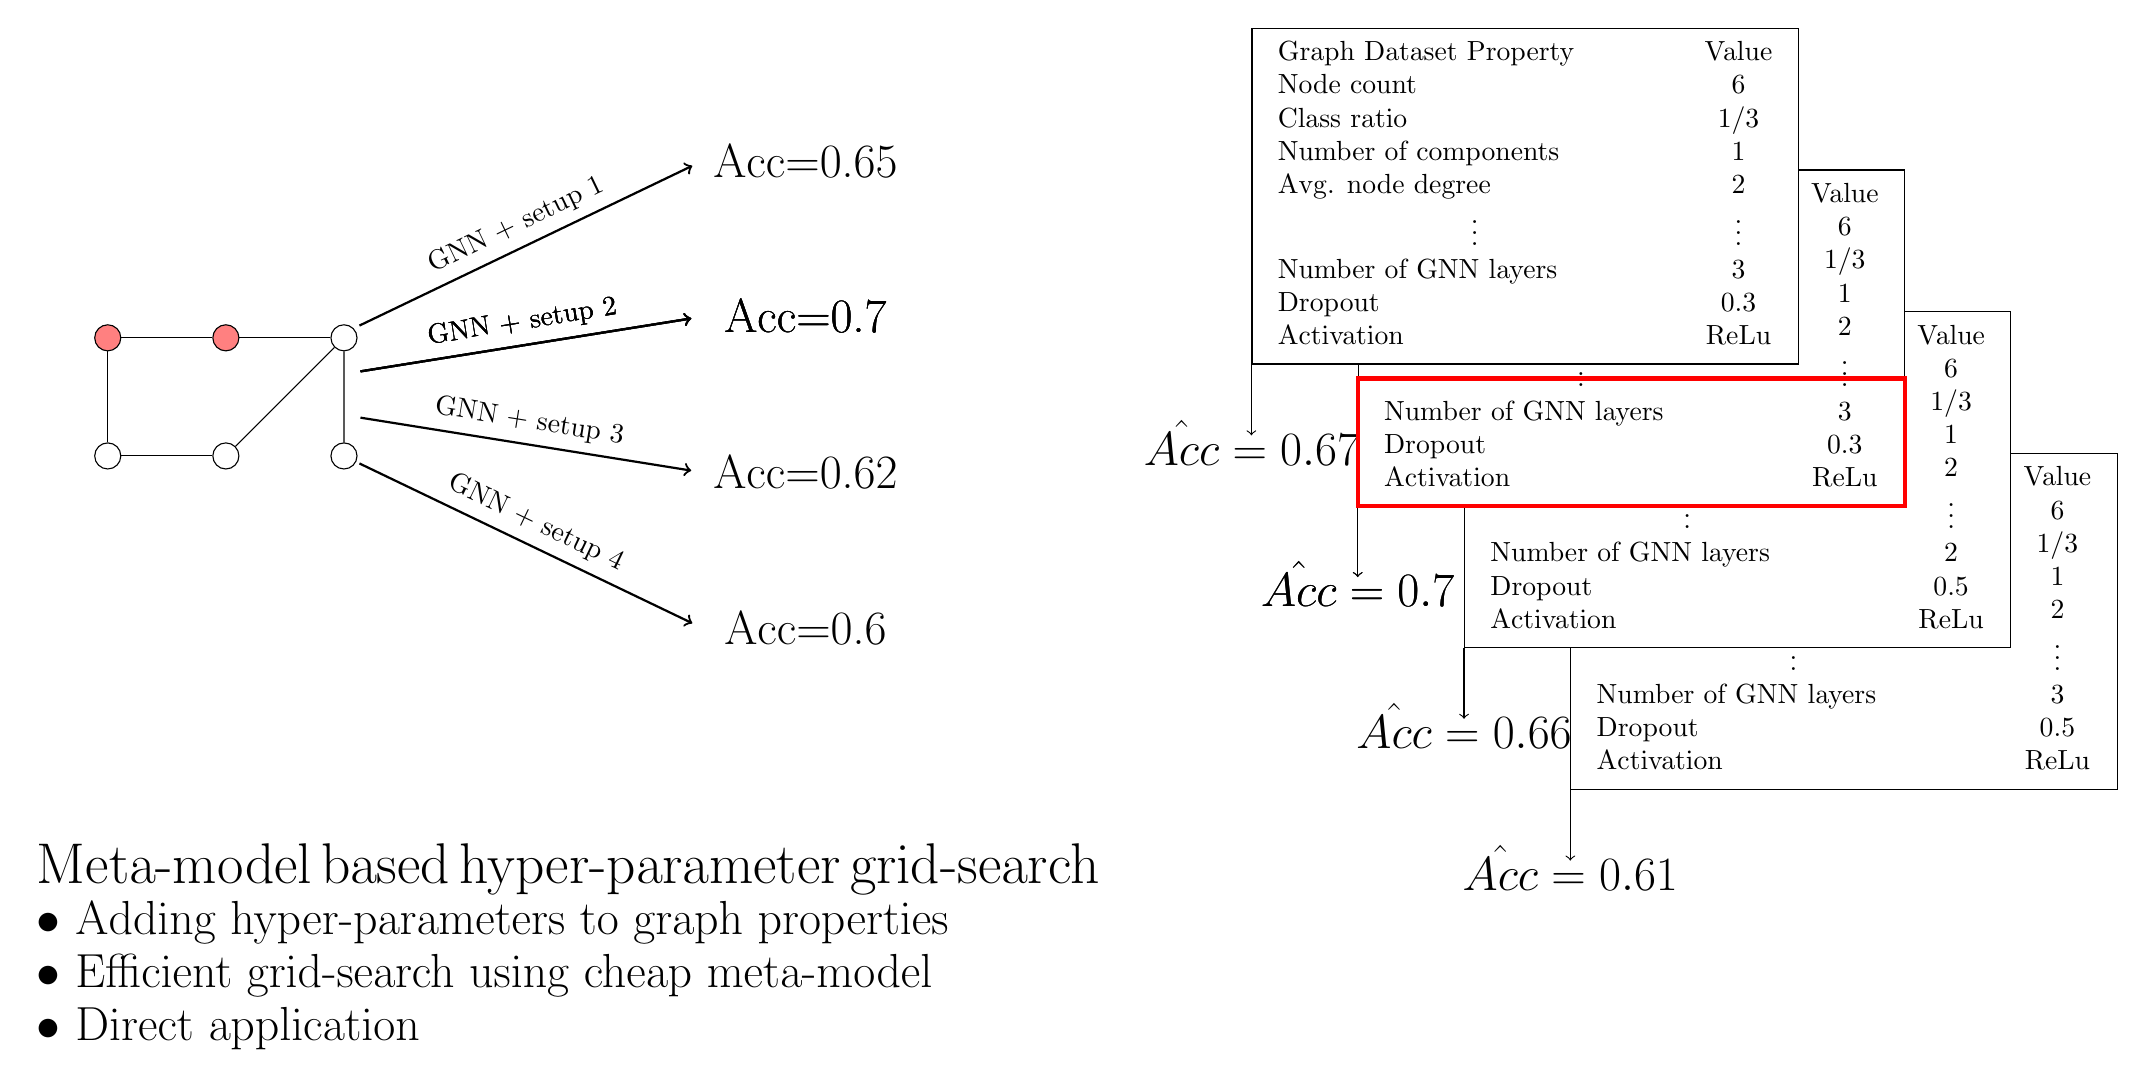
\begin{tikzpicture}[scale=0.9]
\def\dist{1.5cm}
\tikzset{node distance=\dist, minimum size=1ex}

	\tikzset{classA/.style={circle, draw=black, fill=blue!20!yellow}}
	\tikzset{classB/.style={circle, draw=black, fill=blue!20}}
	\tikzset{classC/.style={circle, draw=black, fill=yellow!20!red}}
	\tikzset{class1/.style={circle, draw=black, fill=red!50}}
	\tikzset{class0/.style={circle, draw=black, fill=white}}
	\tikzset{desc/.style={rectangle, anchor=west, text width=2.5cm,minimum height=1cm,minimum width=2.8cm, rounded corners=1ex, align=center}}

	\newcommand{\drawgraph}[9]{
\begin{scope}[xshift=#1, yshift=#2]
\node[#3] (#9A1) {};
\node[#4, right of=#9A1] (#9A2) {};
\node[#5, below of=#9A1] (#9B1) {};
\node[#6, right of=#9A2] (#9B2) {};
\node[#7, below of=#9A2] (#9C1) {};
\node[#8, below of=#9B2] (#9C2) {};
\draw [-] (#9A1) -- (#9A2);
\draw [-] (#9A1) -- (#9B1);
\draw [-] (#9B1) -- (#9C1);
\draw [-] (#9C1) -- (#9B2);
\draw [-] (#9B2) -- (#9C2);
\draw [-] (#9A2) -- (#9B2);
\end{scope}
	}

\drawgraph{-12cm}{7.5cm}{class1}{class1}{class0}{class0}{class0}{class0}{task1}

%\node[fill=white, draw] (r4) at (8, 9.5) {
%    \begin{tabular}{p{5cm}c}
%        Graph Dataset Property & Value  \\
%        \midrule
%        Node count             & 6      \\
%        Class ratio            & 1/3    \\
%        Number of components   & 1      \\
%        Avg. node degree       & 2    \\
%        \centerline{\vdots}    & \vdots \\
%    \end{tabular}};

\uncover<1->{
\draw[->, thick, shorten >=1ex, shorten <=1ex] (-8.6,7.6) -- +(5,2.4) node [pos=0.5, above, sloped] {GNN + setup 1} node [font=\LARGE, pos=1, xshift=1.3cm] {Acc=0.65};

\draw[->, thick, shorten >=1ex, shorten <=1ex] (-8.6,7) -- +(5,0.8) node [pos=0.5, above, sloped] {GNN + setup 2}  node [font=\LARGE, pos=1, xshift=1.3cm] {Acc=0.7};

\draw[->, thick, shorten >=1ex, shorten <=1ex] (-8.6,6.4) -- +(5,-0.8) node [pos=0.5, above, sloped] {GNN + setup 3}  node [font=\LARGE, pos=1, xshift=1.3cm] {Acc=0.62};

\draw[->, thick, shorten >=1ex, shorten <=1ex] (-8.6,5.8) -- +(5,-2.4) node [pos=0.5, above, sloped] {GNN + setup 4}  node [font=\LARGE, pos=1, xshift=1.3cm] {Acc=0.6};


\node[fill=white, draw] (r4) at (12.5, 3.5) {
    \begin{tabular}{p{5cm}c}
        Graph Dataset Property & Value  \\
        \midrule
        Node count             & 6      \\
        Class ratio            & 1/3    \\
        Number of components   & 1      \\
        Avg. node degree       & 2    \\
        \centerline{\vdots}    & \vdots \\
        Number of GNN layers   & 3      \\
        Dropout                & 0.5    \\
        Activation             & ReLu   \\
    \end{tabular}
};

\node[fill=white, draw] (r3) at (11, 5.5) {
    \begin{tabular}{p{5cm}c}
        Graph Dataset Property & Value  \\
        \midrule
        Node count             & 6      \\
        Class ratio            & 1/3    \\
        Number of components   & 1      \\
        Avg. node degree       & 2    \\
        \centerline{\vdots}    & \vdots \\
        Number of GNN layers   & 2      \\
        Dropout                & 0.5    \\
        Activation             & ReLu   \\
    \end{tabular}
};


\node[fill=white, draw] (r2) at (9.5, 7.5) {
    \begin{tabular}{p{5cm}c}
        Graph Dataset Property & Value  \\
        \midrule
        Node count             & 6      \\
        Class ratio            & 1/3    \\
        Number of components   & 1      \\
        Avg. node degree       & 2    \\
        \centerline{\vdots}    & \vdots \\
        Number of GNN layers   & 3      \\
        Dropout                & 0.3    \\
        Activation             & ReLu   \\
    \end{tabular}
};


\node[fill=white, draw] (r1) at (8, 9.5) {
    \begin{tabular}{p{5cm}c}
        Graph Dataset Property & Value  \\
        \midrule
        Node count             & 6      \\
        Class ratio            & 1/3    \\
        Number of components   & 1      \\
        Avg. node degree       & 2    \\
        \centerline{\vdots}    & \vdots \\
        Number of GNN layers   & 3      \\
        Dropout                & 0.3    \\
        Activation             & ReLu   \\
    \end{tabular}
};


\draw[->] (r1.south west) -- node[font=\LARGE,pos=1.1] {$\hat{Acc}=0.67$} ([yshift=-1cm] r1.south west);
\draw[->] (r2.south west) -- node[font=\LARGE,pos=1.1] (mmax) {$\hat{Acc}=0.7$} ([yshift=-1cm] r2.south west);
\draw[->] (r3.south west) -- node[font=\LARGE,pos=1.1] {$\hat{Acc}=0.66$} ([yshift=-1cm] r3.south west);
\draw[->] (r4.south west) -- node[font=\LARGE,pos=1.1] {$\hat{Acc}=0.61$} ([yshift=-1cm] r4.south west);
}
\uncover<2->{
%\draw[color=red, ultra ]  (mmax.center) circle (1.3cm);
\draw[->] (r2.south west) -- node[font=\LARGE,pos=1.1] (mmax) {\alert{$\hat{Acc}=0.7$}}([yshift=-1cm] r2.south west);

\draw[->, thick, shorten >=1ex, shorten <=1ex] (-8.6,7) -- +(5,0.8) node [pos=0.5, above, sloped] {GNN + setup 2}  node [font=\LARGE, pos=1, xshift=1.3cm] {\alert{Acc=0.7}};
}
\uncover<3->{
\draw[color=red, ultra thick]  (r2.south west) rectangle ([yshift=1.8cm] r2.south east);

\draw[->, thick, shorten >=1ex, shorten <=1ex] (-8.6,7) -- +(5,0.8) node [pos=0.5, above, sloped] {GNN + \alert{setup 2}}  node [font=\LARGE, pos=1, xshift=1.3cm] {\alert{Acc=0.7}};
}
\uncover<4>{
    \node[text width=180mm, align=left] at (-3, 0) {
{\huge{Meta-model based hyper-parameter grid-search}}
};
    \node [font=\LARGE, text width=180mm, align=left] (top)    at (-3,-0.75) {$\bullet$ Adding hyper-parameters to graph properties};
    \node [font=\LARGE, text width=180mm, align=left] (middle) at (-3,-1.5)  {$\bullet$ Efficient grid-search using cheap meta-model};
    \node [font=\LARGE, text width=180mm, align=left] (bottom) at (-3,-2.25)  {$\bullet$ Direct application};
}
\end{tikzpicture}
}
